\section{Methodology}

This research employs Design Science Research Methodology (DSRM) to systematically develop and evaluate the TrackMyBills expense tracking system. DSRM provides a rigorous framework for creating and assessing technological artifacts that address identified problems in information systems research.

\subsection{Problem Identification and Motivation}
The initial phase identified Generation Z's significant challenges in manual expense tracking despite widespread digital payment adoption, particularly QRIS usage. Analysis revealed that 84\% of Indonesian university students without financial education fail to maintain expense records, while 78\% with financial education still struggle with systematic tracking. This gap between digital payment adoption and expense management presents a clear opportunity for technological intervention.

\subsection{Define Objectives for Solution}
The research objectives focus on developing a mobile-based expense tracking system that automatically extracts and categorizes financial information from various payment documents using computer vision and deep learning technologies. The system aims to eliminate manual data entry requirements while maintaining high accuracy and providing intuitive user experience specifically designed for Generation Z preferences and behaviors.

\subsection{Design and Development}
This phase represents the core contribution of the research, encompassing model development, system architecture design, and implementation following the 4+1 architectural view model. The development process begins with data preparation and model training, utilizing the CORD-v2 dataset containing 1,000 annotated receipt images for the base model and the QRIS-TF custom dataset comprising 471 Indonesian digital payment confirmation images for the custom model.

The system architecture design follows comprehensive architectural principles to ensure scalability, maintainability, and performance. The TrackMyBills system implements a client-server architecture comprising a Flutter-based mobile application for Generation Z users and a FastAPI-based backend service (DonutAPI) providing OCR-free document processing through fine-tuned Donut transformer models. The architectural design process employs the 4+1 view model to address different stakeholder perspectives and ensure comprehensive system specification.

\subsubsection{Use Case View}
\begin{figure}[htbp]
    \centering
    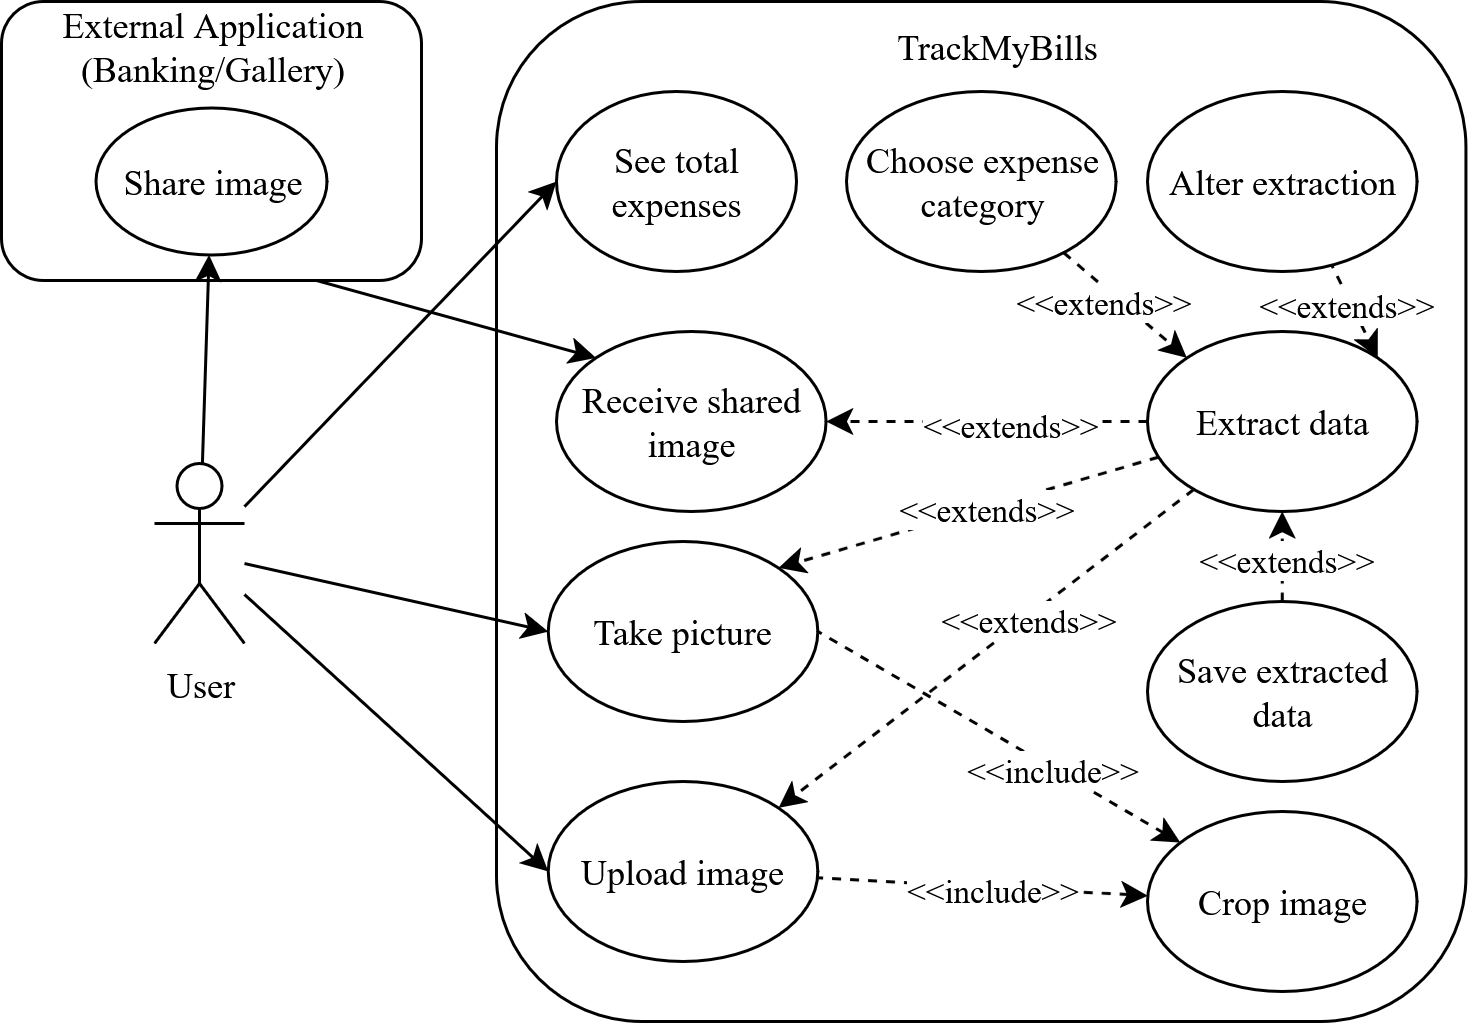
\includegraphics[width=0.48\textwidth]{images/use-case-eng.png}
    \caption{System Use Case Diagram}
    \label{fig:usecase}
\end{figure}

Figure \ref{fig:usecase} illustrates primary user interactions encompassing five distinct workflows: sharing from payment applications, camera capture for paper receipts, gallery upload for existing images, camera capture for digital payments, and upload for digital payment screenshots. The use case view demonstrates comprehensive functionality accommodating various Generation Z usage patterns while maintaining simplicity and intuitive operation. Each use case addresses specific scenarios where users interact with different types of financial documents, ensuring system flexibility and comprehensive coverage of real-world expense tracking situations.

\subsubsection{Logical View}
The logical architecture implements separation of concerns through layered design principles. The presentation layer handles user interface and interaction through Flutter widgets and state management, providing responsive and intuitive interfaces optimized for mobile interaction patterns. The business logic layer processes document analysis requests and manages data transformation between mobile application and backend service, implementing domain-specific rules for financial document processing. The data layer encompasses local SQLite storage for offline capability and remote model inference through RESTful API communication, ensuring data persistence and system reliability across network conditions.

\subsubsection{Process View}

The process view outlines the system's operational workflow, detailing the sequence of interactions between mobile application components and backend services. The TrackMyBills application initiates document processing by capturing images or uploading files, which are then sent to the DonutAPI for analysis. The backend service processes the documents using the appropriate model based on the document type, returning structured data to the mobile application for user display and storage. This process view emphasizes asynchronous communication patterns, ensuring responsive user experiences while maintaining efficient backend processing capabilities.

% Figure \ref{fig:process} demonstrates the comprehensive development methodology from problem identification through system deployment. The process view emphasizes iterative development cycles, systematic testing phases, and continuous integration practices ensuring robust system evolution. The development flow incorporates user feedback integration, performance optimization cycles, and scalability considerations aligned with production deployment requirements. Each development phase includes validation checkpoints and quality assurance measures to maintain system reliability and user experience standards.

\subsubsection{Development View}

Figure \ref{fig:component} presents the component-level architecture detailing interaction patterns between mobile application modules and backend service components. The development view facilitates implementation coordination by specifying component interfaces, dependency relationships, and communication protocols. Key mobile application components include image capture modules, document processing handlers, user interface controllers, and local data management systems. Backend service components encompass model inference engines, API request processors, response formatters, and system monitoring utilities. The component architecture enables modular development, independent testing, and systematic maintenance procedures.

\begin{figure}[htbp]
    \centering
    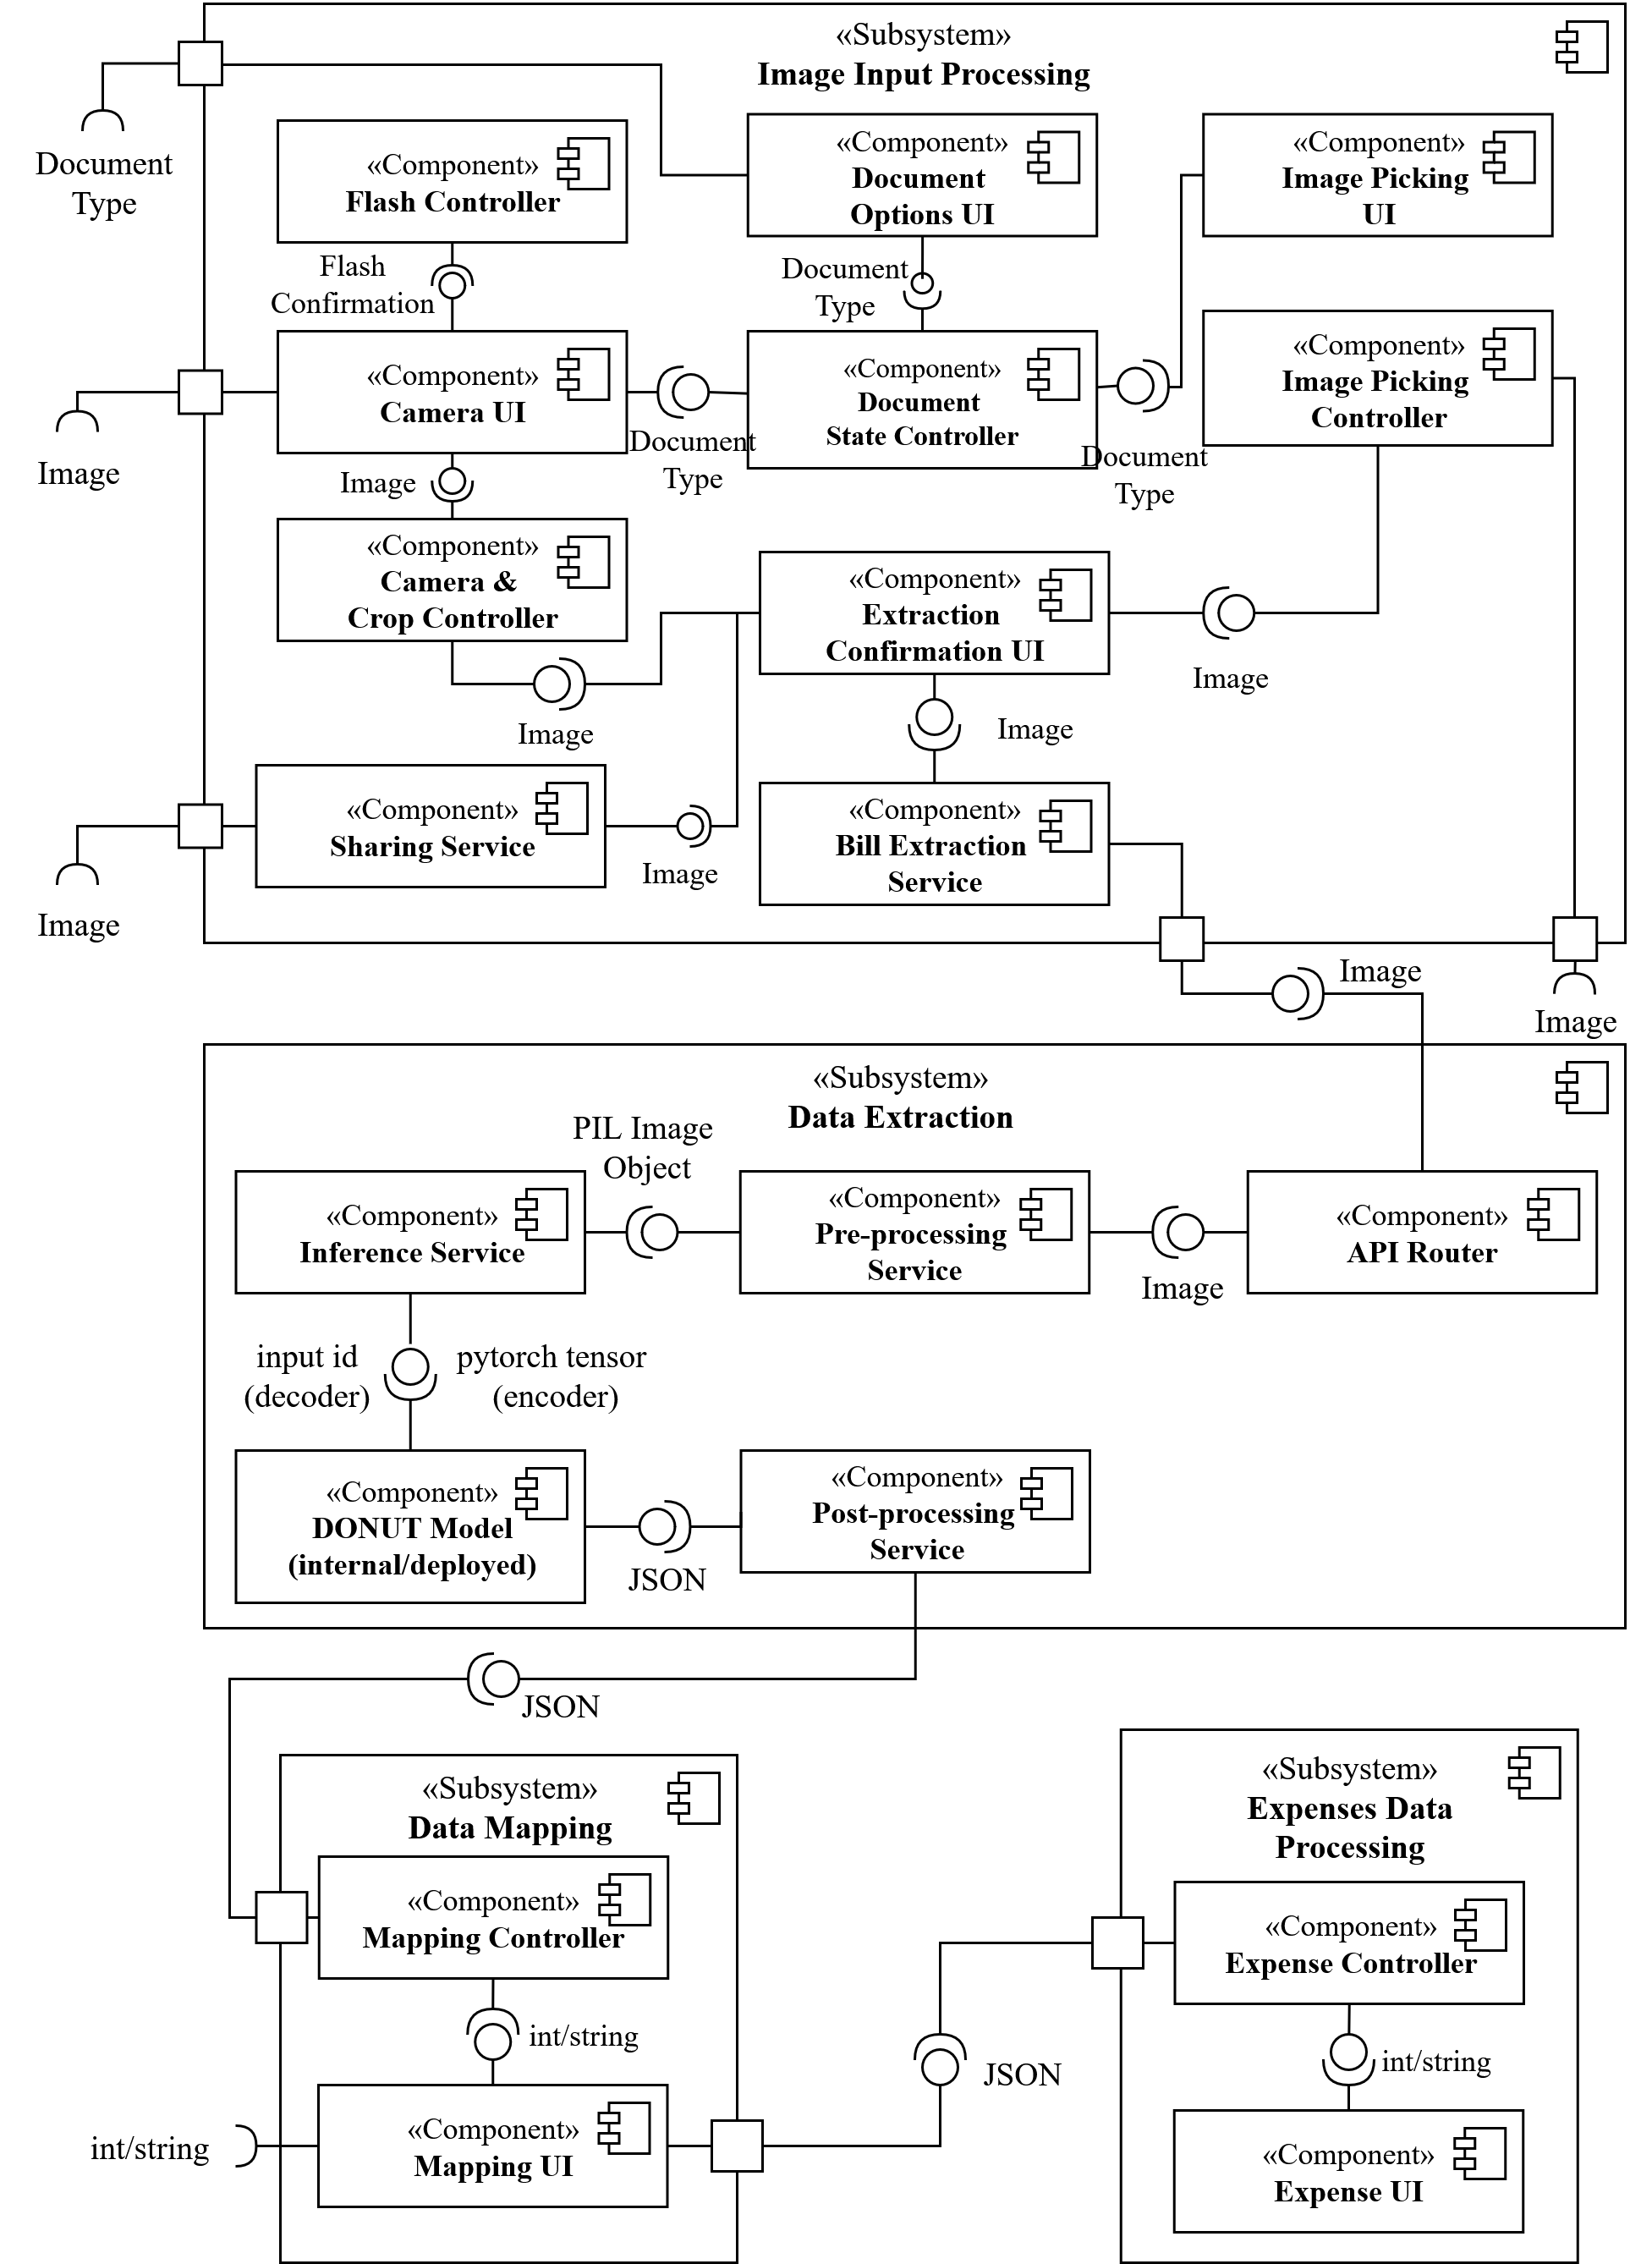
\includegraphics[width=0.48\textwidth]{images/component-diagram-eng.png}
    \caption{Component Architecture Diagram}
    \label{fig:component}
\end{figure}

\subsubsection{Physical View}
The physical architecture addresses deployment and runtime environment considerations for production system operation. The mobile application deploys to Android devices through standard application distribution channels, utilizing device hardware capabilities including camera systems, local storage, and network connectivity. The backend service deploys using containerized architecture ensuring environment consistency and horizontal scalability across cloud infrastructure. Physical deployment implements security protocols through HTTPS communication, authentication mechanisms, and data encryption standards. System monitoring and logging capabilities provide operational visibility and performance optimization feedback for continuous system improvement.

\begin{figure}[htbp]
    \centering
    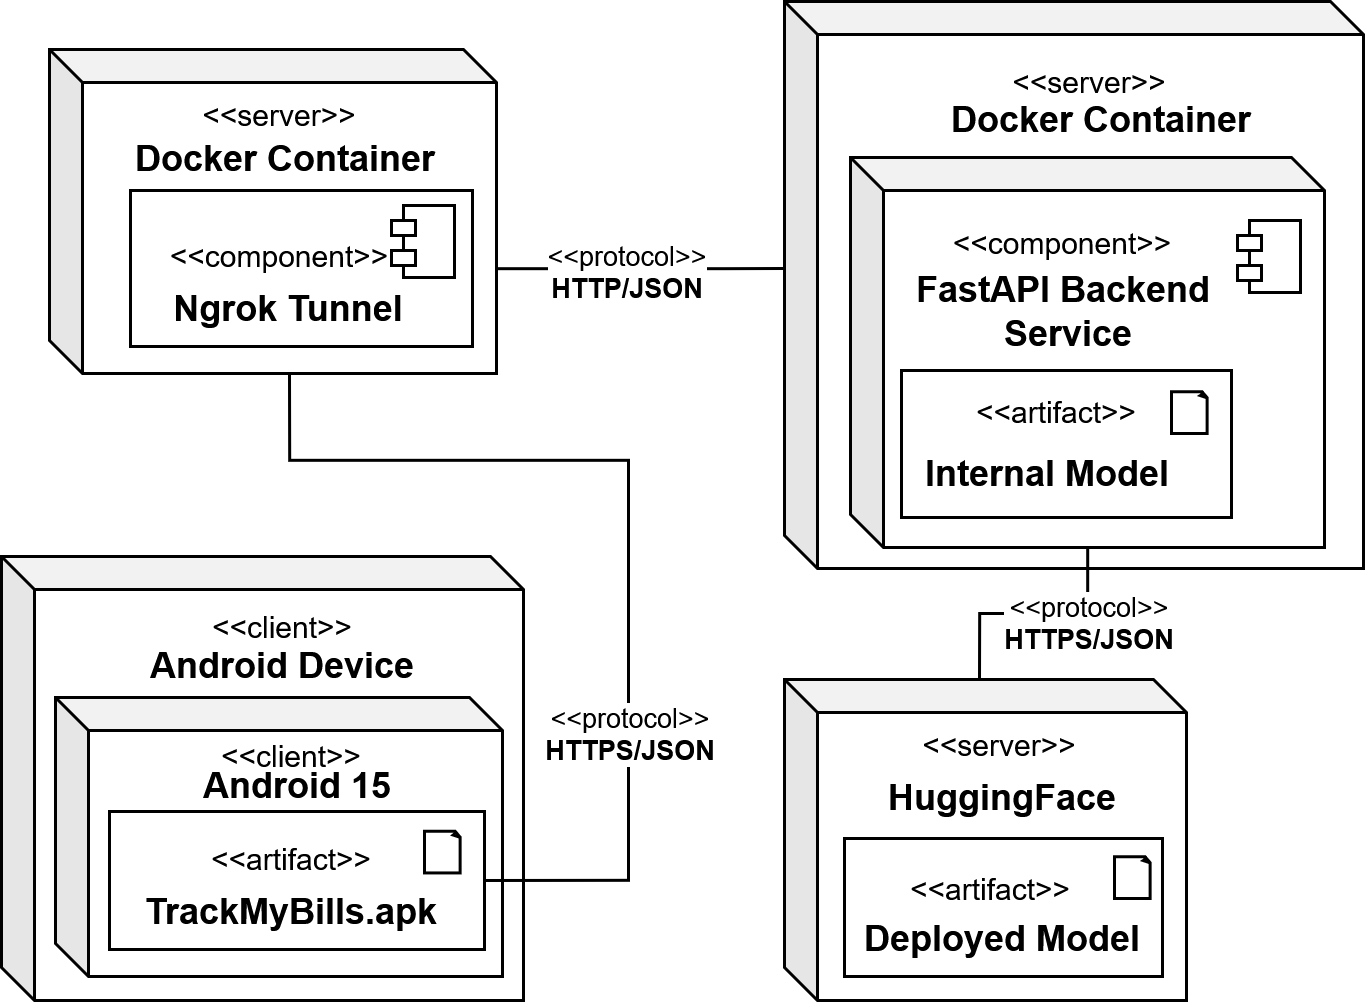
\includegraphics[width=0.48\textwidth]{images/deployment-diagram.png}
    \caption{Deployment Architecture Diagram}
    \label{fig:deployment}
\end{figure}

% \subsubsection{Implementation Architecture}
% The implementation architecture prioritizes mobile-first design principles aligned with Generation Z preferences for seamless, efficient user experiences. The TrackMyBills mobile application implements Clean Architecture patterns with distinct presentation, domain, and data layers enabling maintainable code organization and comprehensive testability. State management utilizes reactive programming principles ensuring responsive user interface updates and consistent application behavior. The DonutAPI backend service provides RESTful endpoints optimized for mobile consumption with automatic model selection, structured JSON responses, and comprehensive error handling. Service architecture implements asynchronous processing patterns, request queuing mechanisms, and response caching strategies to maintain optimal performance under varying load conditions.

\subsection{Demonstration}
The demonstration phase validates system functionality through comprehensive testing scenarios covering all five user workflows. Testing encompasses various document types, image qualities, and user interaction patterns to ensure robust system performance across diverse real-world conditions. Each workflow undergoes systematic validation to verify end-to-end functionality and user experience consistency. Demonstration activities include functional testing, performance benchmarking, and user acceptance validation with Generation Z participants.

\subsection{Evaluation}
Evaluation employs a multi-dimensional approach assessing model performance, system functionality, and user experience. Model evaluation utilizes standard information extraction metrics including Accuracy, Precision, Recall, F1-score, and mean Character Error Rate (mCER) providing comprehensive assessment of extraction quality. User experience evaluation employs the System Usability Scale (SUS) methodology providing quantitative assessment of interface effectiveness and user satisfaction specifically targeting Generation Z users. The evaluation framework ensures objective measurement of system effectiveness and user acceptance.

\subsection{Communication}
The communication phase disseminates research findings through academic publication and system demonstration. This includes comprehensive documentation of methodology, implementation details, evaluation results, and recommendations for future development. The communication strategy ensures knowledge transfer and enables replication and extension of the research contributions within the academic and professional communities.